% Author: Giulio Stramondo, Mail: giuliostramondo[at]gmail.com
\documentclass{standalone}
\usepackage{tikz}
\usetikzlibrary{positioning,arrows,patterns}
\begin{document}
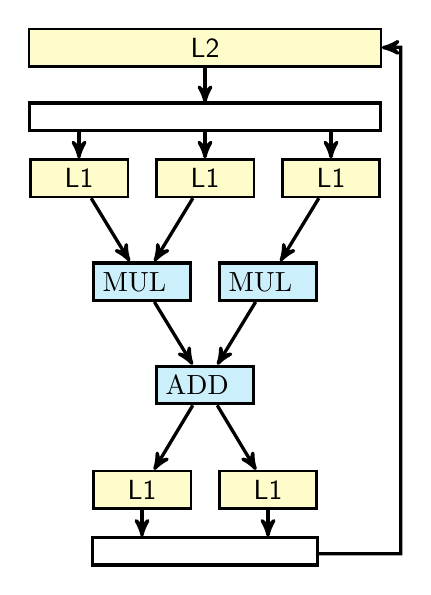
\begin{tikzpicture}[
    archr/.style={rectangle,thick,draw,fill=red!60,anchor=north,
		minimum width=0.2cm},
    archb/.style={rectangle,thick,draw,fill=blue!60,anchor=north,
		minimum width=0.2cm},
    archm/.style={rectangle,thick,draw,fill=magenta!60,anchor=north,
		minimum width=0.2cm},
    select/.style={circle,thick,draw,anchor=north,
		minimum width=0.4cm},
% Event style
    event/.style={rectangle,thick,draw,fill=yellow!20,text width=2cm,
		text centered,font=\sffamily,anchor=north},
%  For compatability with PGF CVS add the absolute option:
   absolute
    ]
%%% Draw system flow diagram
   \begin{scope}[xshift=-7.5cm,yshift=-5cm,very thick,
		node distance=1.6cm,on grid,>=stealth',
		block/.style={rectangle,draw,fill=cyan!20}]
      \node [event, text width =1cm] (l11)  {L1};
      \node [event, text width = 1cm] [right=of l11] (l12)  {L1};
      \node [event, text width = 1cm ] [right=of l12] (l13)  {L1};
      \draw [-,opacity=0] (l11) -- (l12)
       node [pos=1/2] (l1mid12) {};
      \draw [-,opacity=0] (l12) -- (l13)
       node [pos=1/2] (l1mid23) {};
       \node [block, below=of l1mid12, below=30pt, text width =1cm] (mul1)  {MUL};
       \node [block,below=of l1mid23, below=30pt ,text width =1cm] (mul2)  {MUL};
      \draw [-,opacity=0] (mul1) -- (mul2)
       node [pos=1/2] (midmul12) {};
       \node [block,below=of midmul12, below=30pt ,text width =1cm] (add1)  {ADD};
       \node [event,below=of mul1, below=68pt ,text width =1cm] (s1)  {L1};
       \node [event,below=of mul2, below=68pt ,text width =1cm] (s2)  {L1};

       \draw [draw=black] ([yshift= 20pt]l11.north west) rectangle ([yshift=10pt]l13.north east);
       \draw [-,opacity=0] ([yshift=10pt]l11.north west) -- ([yshift=10pt]l13.north east)
            node [pos=1/2] (cbl1mid){};
       \node [] [above=of l11,above=11pt] (cbl11) {};
       \node [] [above=of l12,above=11pt] (cbl12) {};
       \node [] [above=of l13,above=11pt] (cbl13) {};
       \node [] [below=of s1,below=11pt] (cbs1) {};
       \node [] [below=of s2,below=11pt] (cbs2) {};
       \node [] [below=of s2.south east,below=12pt] (cbl2) {};
       \draw [-,opacity=0] ([yshift=20pt]l11.north west) -- ([yshift=20pt]l13.north east)
            node [pos=1/2] (cbl2mid){};
       \draw [draw=black] ([yshift= -20pt]s1.south west) rectangle ([yshift=-10pt]s2.south east);

       \node [event,above=of l12,above=40pt,minimum width = 127pt] (l2) {L2};

       \draw [->] (l2) -- (cbl2mid.center);
       \draw [->] ([yshift=2pt]cbl11.center) -- (l11);
       \draw [->] ([yshift=2pt]cbl12.center) -- (l12);
       \draw [->] ([yshift=2pt]cbl13.center) -- (l13);

       
       \draw [->] (l11) -- (mul1);
       \draw [->] (l12) -- (mul1);
       %\draw [->] (l12) -- (mul2);
       \draw [->] (l13) -- (mul2);


       \draw [->] (mul1) -- (add1);
       \draw [->] (mul2) -- (add1);

       \draw [->] (add1) -- (s1);
       \draw [->] (add1) -- (s2);


       \draw [->] (s1) -- ([yshift=-2pt]cbs1.center);
       \draw [->] (s2) -- ([yshift=-2pt]cbs2.center);

       \draw [->] (cbl2.center) -- ++(30pt,0) -- ++ (0,183pt) -- (l2.east);
   \end{scope}
\end{tikzpicture}
\end{document}

